In this chapter we evaluate DaisyNFS and GoTxn in terms of performance
(\cref{sec:eval:perf}), correctness (\cref{sec:eval:testing}),
and ease of change (\cref{sec:eval:incremental}).

\section{Performance}
\label{sec:eval:perf}

The first question answered by the evaluation is, can DaisyNFS and GoTxn achieve
good performance, compared to an unverified baseline? This section evaluates
performance both with a single and multiple clients.

\subsection{Experimental setup}

To evaluate the performance of DaisyNFS, we ran three benchmarks: the LFS smallfile
and largefile benchmarks, and a development workload that consists of \cc{git
clone} from a local repository followed by running \cc{make}. These are the same
benchmarks used by DFSCQ~\cite{chen:dfscq} (a state-of-the art sequential
verified file system). As a baseline, this evaluation compares against a Linux
NFS server exporting the widely-used ext4 file system.
The NFS server lets us compare fairly since both go through the Linux NFS client
and use the same underlying protocol. The ext4 file system is run in the
non-default \cc{data=journal} mode, forces all data to
go through the journal and disables log-bypass writes, which gives the same
crash-safety guarantees and makes the designs more comparable. In its default
\cc{data=ordered} mode Linux achieves better performance on some benchmarks but
can lose recently written data if the system crashes; we also present some results to
show the benefit of providing this weaker guarantee.

All of these benchmarks were run using Linux~5.13, Dafny~3.5.0, Go~1.18.1 on an Amazon
EC2 i3.metal instance, which has two 36-core Xeon processors running at 2.7~GHz, 512~GB of RAM, and a local 1.9~TB
NVMe SSD.\@ To reduce variability we use a bare-metal instance, limit experiments to a single 36-core
socket, disable turbo boost, and disable processor sleep states; the coefficient
of variation for all experiments is under 5\% so we omit error bars for visual
clarity.

The three benchmarks test different aspects of file system performance:

\paragraph{Smallfile.}
The smallfile benchmark is a metadata-heavy benchmark that repeatedly creates a
file, writes 100 bytes to it, calls \cc{fsync()}, and then deletes the file. The
performance reported is the throughput in terms of files/s for this whole process. At
the NFS level each iteration results in four RPCs issued to the server: \cc{LOOKUP} for the file
being created (which fails), \cc{CREATE}, \cc{WRITE}, and \cc{REMOVE}. Because
both systems run the same RPCs, the comparison is meaningful.

The smallfile benchmark is also used to measure the scalability of the file
system. We run several concurrent clients, each repeatedly running the
create-write-delete sequence above, for several seconds, then report the
aggregate throughput of all of these clients. A concurrent file system should be
able to process these RPCs simultaneously --- concurrent threads have a chance
to prepare new transactions while the system is committing older transactions.
Furthermore on a physical disk the journaling for simultaneous operations can be
combined (an optimization called \emph{group commit}), resulting in less I/O
than separate commits.

\paragraph{Largefile.}
The largefile benchmark is a data-heavy benchmark that creates a file, then
repeatedly appends to the file until it is 300 MB, and finally calls
\cc{fsync()} and closes the file. The performance reported is the throughput in
terms of MB/s for these appends. The Linux NFS client buffers the entire append
process until the final sync, at which point it issues the writes in many chunks
in parallel. This benchmark is challenging to support efficiently because the
writes at the NFS server do not come in order, so some are past the end of the
file and then the gap is filled in by later RPCs.

\paragraph{App.}
The application workload ``app'' consists of running \cc{git clone} on the xv6
repository followed by \cc{make}. The main purpose of including this workload is to
demonstrate that DaisyNFS covers a useful range of the NFS interface, since
\cc{git clone} especially uses a wider mix of operations and arguments than the
other benchmarks, and also that the file system implements these operations
efficiently enough to not slow down the workload. The performance reported for
app converts this latency to a throughput number ``app/s'' so that higher is
better. The compilation part of this workload does take about 1.2s, out of an
overall build that typically takes about 2.5s under Linux NFS, and this time is
unaffected by the file system's performance.\@ The xv6 code being compiled is an
operating system, so building it requires running the usual development
tools---gcc, ld, ar---but also running dd to generate a kernel image.

\subsection{Single-client performance}

%% cpupower frequency-set -g performance
%% threads=32 in the [nfsd] section of /etc/nfs.conf

%% SINGLE-CORE EXPERIMENTS:
%%   for n in $(seq 8 15) $(seq 24 31); do echo 0 > /sys/devices/system/cpu/cpu$n/online; done

\begin{figure}[ht]
  \centering
  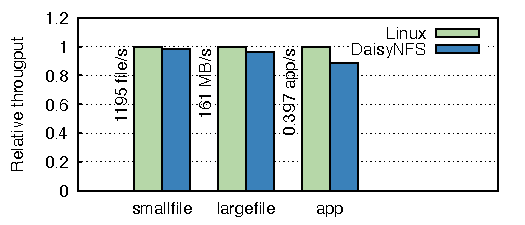
\includegraphics{daisy-nfs/fig/bench.pdf}
  \caption[Performance for smallfile, largefile, and app benchmarks]%
  {Performance of Linux NFS and DaisyNFS for \cc{smallfile},
    \cc{largefile}, and \cc{app} workloads, on an in-memory disk.
    DaisyNFS achieves comparable performance to Linux across these benchmarks.}
  \label{fig:eval:bench}
\end{figure}

The first set of results are for the three benchmarks, run on an in-memory disk, all
with a single client. These benchmarks are challenging to support efficiently
since an in-memory disk means performance isn't dominated by slow I/O, and a
single client demands single-core efficiency.
The results are shown in \cref{fig:eval:bench}. DaisyNFS achieves
comparable performance on these benchmarks after implementing many optimizations
(for example, parsing data structures in-place) and features (for example,
returning attributes to enable client-side caching). Both CPU and I/O efficiency
are important to get good performance.

DaisyNFS gets slightly lower throughput compared to Linux on the largefile
benchmark. The NFS client's behavior on
this benchmark means it issues writes past the end of the file; the semantics of
such a write are to fill the gap with zeros. DaisyNFS and Linux get good
performance despite this because they implicitly encode those zeros without even
allocating a block. This benchmark shows that GoTxn is good at handling
concurrent, synchronous writes.

\subsection{Scalability}

The next experiment evaluates DaisyNFS's scalability by measuring the throughput
when clients issue operations concurrently. The benchmark used is the smallfile
benchmark with a varying number of concurrent clients, all running in separate
directories. Because this experiment runs on a physical disk, other threads have
a chance to prepare transactions while the transaction system is committing to
disk.

To evaluate the importance of DaisyNFS's concurrency, we compare against two
other configurations of DaisyNFS with reduced concurrency. The ``seq WAL'' configuration
adds locks to the write-ahead log so that the disk operations that normally
execute lock-free --- installation, logging, and reading installed data ---
instead happen under the write-ahead log's in-memory lock. This permits
transactions to execute concurrently while not accessing GoTxn but does not
allow any parallel disk access. The ``seq txn'' variant leaves the write-ahead
log the same but changes the per-address locking in GoTxn to a \emph{global}
transaction lock, preventing any transactions from running concurrently but
allowing concurrency between logging and installation in the write-ahead log.

\begin{figure}[ht]
  \centering
  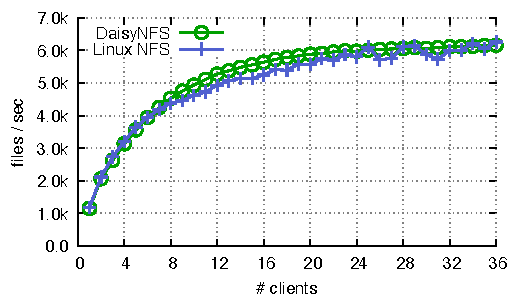
\includegraphics{daisy-nfs/fig/scale.pdf}
  \vspace{0.5\baselineskip}
  \caption[Concurrent smallfile performance]%
  {Combined throughput of the \cc{smallfile} microbenchmark, varying the number
    of concurrent clients. DaisyNFS's performance scales with the number of
    clients, but both eventually scale sub-linearly due to lock contention. DaisyNFS has a single lock that becomes contended more quickly than the contention observed in Linux.}
  \label{fig:eval:scale}
\end{figure}

% \begin{figure}[hp]
%   \includegraphics{daisy-nfs/fig/scale-ram.pdf}
%   \caption[Concurrent smallfile performance, with RAM disk]%
%   {Combined throughput of the \cc{smallfile} microbenchmark running on an
%     in-memory disk while varying the number of concurrent clients.}
%   \label{fig:eval:scale-ram}
% \end{figure}

\paragraph{Scaling with number of clients.}

The scalability experiment varies the number of concurrent smallfile clients,
measuring the aggregate throughput of all of the clients. The results are shown in \cref{fig:eval:scale}. Each data point is the
result of running for 30 seconds. The graph shows that both DaisyNFS and Linux
achieve better performance as the number of clients increase, though Linux has
better scalability on this benchmark. The peak throughput of DaisyNFS is about
60\% of the throughput of Linux.

With a large number of clients, both file systems
stop scaling due to lock contention; they are neither I/O bottlenecked nor are
they using the entire CPU.\@ For example, with 30 clients Linux uses only 19\% CPU
while DaisyNFS uses 19\% in userspace and an additional 8\% in the kernel; both
numbers include the cost of the NFS client, which runs in the kernel. We
confirmed that I/O is not a bottleneck with an analogous experiment run on an in-memory disk, shown in \cref{fig:eval:scale:ram}. DaisyNFS has a common
lock for installing sub-block object writes into a full block, which all
operations go through to commit. The Go mutex profile points to this lock as
being the biggest source of contention in DaisyNFS for both the NVMe and
in-memory benchmarks. The fact that scalability is limited by this common lock indicates the importance of concurrency for performance.

\begin{figure}[ht]
  \centering
  \includegraphics{daisy-nfs/fig/scale-ram.pdf}
  \vspace{0.5\baselineskip}
  \caption[Concurrent smallfile performance on in-memory disk]%
  {Scalability on the \cc{smallfile} benchmark, running on an in-memory disk.}
  \label{fig:eval:scale:ram}
\end{figure}


The DaisyNFS seq WAL and seq txn variants show even more clearly that
concurrency is important for performance. In both configurations, throughput
essentially doesn't increase beyond two clients. Going from one to two clients
helps because even though in
both of these configurations the server cannot process more than one request at
a time, performance improves slightly with a second client since a request can
be received while another is being processed.

\paragraph{Concurrency and log bypass for largefile.}

\begin{figure}[hp]
  \begin{subfigure}[b]{\textwidth}
    \includegraphics{daisy-nfs/fig/extended-bench.pdf}
    \caption{On an NVMe disk}
    \label{fig:bench-configs:nvme}
  \end{subfigure}

  \begin{subfigure}[b]{\textwidth}
    \includegraphics{daisy-nfs/fig/extended-bench-ram.pdf}
    \caption{On an in-memory disk}
    \label{fig:bench-configs:ram}
  \end{subfigure}
  \vspace{0.5\baselineskip}
  \caption[Benchmarks across file-system configurations]%
  {Performance across various file-system configurations. The smallfile
    benchmark is run with a single client (\cc{smallfile-1}) and also with 25
    parallel clients (\cc{smallfile-25}). The ``log bypass'' variant of Linux
    uses the \cc{data=ordered} to write data directly rather than through the
    journal. The ``seq txn'' variant of DaisyNFS has a global transaction lock
    while ``seq WAL'' adds additional locking to the write-ahead log.}
  \label{fig:bench-configs}
\end{figure}

The final set of experiments aims to understand the performance of DaisyNFS on
the largefile and app benchmarks as well. We compare against the same variants
of DaisyNFS with reduced concurrency, as well as against Linux with its
log-bypass optimization (that is, \cc{data=journal} mode).
The results are presented in \cref{fig:bench-configs},
on both an NVMe disk and an in-memory disk. The results for the NVMe disk have
most of the interesting trends, but there are a few interesting differences
worth noting.

The \cc{smallfile-25} and \cc{smallfile-1} numbers repeat individual points from
the \cref{fig:eval:scale}, but presented as throughput relative to Linux so that
it is easier to compare across file systems. The \cc{smallfile-1} results shown
here make it clearer that DaisyNFS has worse performance than Linux with
only a single client on a physical disk, even though performance is comparable with an in-memory disk. This is due to less efficient use of
the NVMe drive; looking at the kernel's I/O statistics, both file systems have
similar total disk bandwidth (130 MB/s for Linux and 120 MB/s for DaisyNFS), but
DaisyNFS's I/O patterns result in about 4KB I/O requests which have higher
latency than with Linux. DaisyNFS spends most of its time waiting on disk I/O in
this benchmark. \tej{can still double-check this by looking at the addresses
being written with \cc{blktrace}}

The \cc{smallfile-1} benchmark is interesting because the client issues a single
operation at a time, and yet seq WAL performs noticeably worse. This is because
the write-ahead log is parallelizing logging writes and installing them to the
disk (rather than alternating between logging and installation), and the disk is
able to get better throughput by doing these concurrently.

On the \cc{smallfile-25} benchmark DaisyNFS can coalesce concurrent operations
and journal them together to reduce total I/O. Unlike with \cc{smallfile-1},
lock contention dominates I/O performance so both file systems perform similarly
between disk and memory (even in absolute performance).

The \cc{largefile} benchmark is interesting because the client issues many
concurrent operations, but they all conflict since they write to the same file.
Linux and DaisyNFS handle this contention fine, still achieving good throughput
given that all writes have to be written to both the journal and data region in
both systems. However, we can see that a global txn lock actually performs
\emph{better} than the per-address locking, showing a case where with enough
conflicts two-phase locking has some overhead compared to a simpler locking
scheme. The seq WAL case achieves lower performance for similar reasons to
smallfile-1, since it again alternates logging and installation rather than
issues them concurrently.

The \cc{app} benchmark is less heavy on writes, and its performance
is barely affected by concurrency in DaisyNFS.

Another comparison shown in the same figure is to Linux with its log bypass
optimization (the default \cc{data=ordered} mode), where writes can be written
directly to a file's data blocks rather than going through the journal. This optimization
makes a difference only for asynchronous (``unstable'') NFS writes, since synchronous writes
are journaled even with this option. The smallfile benchmark has only
synchronous writes, so unsurprisingly performance is the same, but on the
largefile benchmark Linux with log bypass achieves 80\% higher throughput. An
improvement of up to $2\times$ better throughput is expected here since unlike
in all the other configurations, data writes are written only once rather than
to both the journal and the data region, and the actual benefit is high since
the benchmark is dominated by disk writes. It's worth noting that even Linux
does not saturate the disk, which can achieve 500 MB/s in sequential write
throughput, due to the overhead of running over NFS.

The log bypass optimization has been verified in prior work on
DFSCQ~\cite{chen:dfscq}, a verified sequential file system. While the
optimization is not out of reach for verification in Perennial, it does break
the GoTxn abstraction boundary, since log bypass writes are not persisted
together with other writes in a transaction. What is much more achievable is
transactions with asynchronous or deferred durability, where the writes are
visible after commit but persisted only later. This optimization does not make
much difference for the \cc{largefile} benchmark because the write size is
large, but it is useful to combine several small writes in memory into one large
transaction.

\section{Testing the trusted code and spec}
\label{sec:eval:testing}

This section answers the question, what are the trusted (assumed correct)
aspects of the DaisyNFS correctness theorem? It also discusses what we did to
use testing to improve confidence in these components.

For the proof of \cref{thm:daisy-correctness-restatement} to apply to the actual server, we trust that (1) the
Dafny code is a ``safe'' use of the transaction system, (2) sequential
refinement is correctly encoded into Dafny, (3) the libraries for Go primitives
are correctly specified in Dafny, and (4) the unverified Go code calling the
Dafny methods and implementing the NFS wire protocol is correct. The
user must follow the assumed execution model and run initialization from an
empty disk and recovery after each boot. Finally, the disk needs to behave
according to its assumed specification, which requires that it preserve written
data and not corrupt it.

Beyond satisfying this formal theorem statement, we want two more things from
the implementation and specification: first that the specification as formalized
actually reflects the RFC, and second we would like DaisyNFS to be compatible
with existing clients, including implementing enough of the RFC's functionality.
These fall outside the scope of verification so we cover them with testing.

To evaluate the file system's correctness and compatibility as a whole, we
mounted it using the Linux NFS client and ran the fsstress and fsx-linux tests,
two suites used for testing the Linux kernel. In order to look for bugs in crash
safety and recovery, we also ran CrashMonkey~\cite{mohan:crashmonkey}, which
found no bugs after running all supported 2-operation tests.

While other experiments in the evaluation interact with DaisyNFS via the Linux
client, these tests interact with the server directly from a hand-written
client. That client is then tested with symbolic execution over the entire server.
This testing produces a wider range of requests than are possible via the Linux
client. The process helped us find and fix several bugs in the unverified parts
of DaisyNFS and in the specification itself, which are reported in
\cref{fig:daisynfs-bugs}.

Most of the bugs in unverified code were bugs in parsing and were readily caught
by symbolic execution. The bug when attempting to call REMOVE on a directory was
a type-safety issue in an untested code path, which was not caught statically
due to limitations in the Go type system. The concurrent write issue is
a particularly interesting bug in unverified code. It only triggered when using
asynchronous writes (which are unverified), but the symptom was that \cc{git
clone} resulted in incorrect data and git complained about consistency errors.
The issue was that the unverified code directly passed a byte slice with the
\cc{WRITE} data from the RPC library into DaisyNFS. This buffer went through the
entire stack and was eventually passed to GoTxn, which retains the buffer.
Unfortunately the RPC library \emph{also} re-uses the buffers that hold network
requests, and eventually the buffer was corrupted due to a concurrent request.
We fixed the bug by copying from the RPC before passing the buffer to the Dafny
code. The subtle aspect of this bug is that it is the ownership implicit in the
Dafny specification that was violated by the surrounding code, not a
straightforward precondition.

Two of the specification bugs are particularly interesting. The bounded inode bug
was due to an \cc{ino} argument of type \cc{Ino}; this type is a Dafny
\emph{subset type}, thus adding an implicit precondition that \cc{ino <
NUM_INODES}, which can be violated by the (unverified) Go code. The fix is to instead
use a \cc{uint64} and check the bound in verified code. The RENAME bug was due
to having an incomplete specification (and implementation) that did not capture
that RENAME should only overwrite when the source and destination are
compatible.

\begin{figure}
  \begin{center}
  \begin{tabular}{@{}p{8cm}p{2.7cm}@{}}
    \toprule
    \textbf{Bug} & \textbf{Why?} \\
    \midrule
    XDR decoder for strings can allocate $2^{32}$ bytes & Unverified \\
    File handle parser panics if wrong length & Unverified \\
    WRITE panics if not enough input bytes & Unverified \\
    Directory REMOVE panics in dynamic type cast & Unverified \\
    Panic on unexpected enum value & Unverified \\
    Concurrent writes can conflict & Unverified \\
    The names \cc{.} and \cc{..} are allowed & Not in RFC 1813 \\
    RENAME can create circular directories & Not in RFC 1813 \\
    CREATE/MKDIR allow empty name & Specification \\
    Proof assumes caller provides bounded inode & Specification \\
    RENAME allows overwrite where spec does not & Specification \\
    \bottomrule
  \end{tabular}
  \end{center}
  \caption{Bugs found by testing at the NFS protocol level.}
  \label{fig:daisynfs-bugs}
\end{figure}

%As a sanity check on the transaction system, we fuzzed the interface presented
%to Dafny using a test harness capable of performing arbitrary reads, writes and
%commits while following the transaction system's preconditions. The test checks
%that the transaction system does not crash and returns the correct data on read.
%The fuzzing did generate complex inputs with multiple chained operations but did
%not find any bugs, but we note that our fuzzing is limited to
%single-threaded and crash-free behavior. \joe{I think we could cut this para now, or perhaps make it more focused by saying it's about testing the trusted boundary between Dafny and GoTxn. But I'm not quite sure it actually does test that?}

\section{Incremental improvements}
\label{sec:eval:incremental}

This section answers the question, how difficult was it to make improvements to
the code and update the proofs? Put more broadly, what is the experience of
making incremental changes to the proof?

DaisyNFS was implemented and verified over the course of three months by the
thesis author, until it had support for enough of NFS to run. We
added several features incrementally after the initial prototype
worked, both to improve performance and to support more
functionality. Some of the interesting changes are listed in
\cref{fig:features}.  To improve performance, we switched to
operating on the serialized representation of directories directly
(decoding fields on demand and encoding in-place) and then added also
multi-block directories.  We added support for attributes so that the file
system stores the mode, uid/gid, and modification timestamp for files and directories.
Finally, we implemented the freeing plan described
in \cref{sec:dafny:freeing}, which required additional code through the
whole stack (but by design no changes to the file-system invariant).
We believe additional features such as symbolic links
could be added incrementally with modest effort because
of sequential reasoning and proof automation.

\begin{figure}[ht!]
\begin{center}
\begin{tabular}{lrr}
  \toprule
  \textbf{Feature} & \textbf{Time} & \textbf{Lines} \\
  \midrule
  In-place directory updates & 2 days & 600\\
  Multi-block directories & 5 days & 800 \\
  NFS attributes & 4 days & 500 \\
  Freeing space (\cref{sec:dafny:freeing}) & 3 days & 1400\\
  \bottomrule
\end{tabular}
\end{center}
\caption{Incremental improvements to the file-system code were implemented
  quickly and without much code (which includes both implementation and proof).}
\label{fig:features}
\end{figure}

For the smallfile benchmark, it took some work to ensure that the Linux NFS
client issued exactly four RPCs per iteration. What this involved was returning
the correct ``weak cache-consistency'' data from all operations, so that the
client reliably caches attribute information. The RFC says these post-operation
attributes are optional but encouraged for the server, but without this
information in practice the Linux client issues additional \cc{GETATTR} and
\cc{ACCESS} RPCs, significantly slowing down DaisyNFS. A big part of the
performance improvement while developing DaisyNFS involved returning more
attribute information, and at the same time expanding the specifications to say
the additional metadata is correct. These improvements were carried out in many
small steps, but they were similar to the incremental improvements above in
terms of taking a small amount of time and few changes to lines of proof; most
of the work went into figuring out what was missing in the implementation.

GoTxn had fewer incremental changes to the code and proof after its initial
development. Three changes are worth noting. First, the write-ahead log was
split into three components: the on-disk circular buffer, the in-memory data
structure caching the log, and finally the rest of the code integrating these
components. This organization become clear while writing the specification and
thinking about the proof. The write-ahead log is the largest single library in
GoTxn, with the largest lines of code even after splitting off these two data
structures, so factoring its complexity was essential to the proof. The second
change was an optimization Mark Theng made to improve performance. Installation
absorbed multiple writes to the same address before installing as a way of
simplifying the proof, but Mark found this hurt performance since typically absorption had already ocurred earlier, and the process had a non-trivial CPU cost. He was able to
eliminate it and fix the proof; notably this change incrementally changed an
already-complete proof. Finally, the transactional part of GoTxn implemented
with two-phase locking was a later idea,
which pleasantly enough was verified on top of the existing lifting-based
journaling specification without any changes to the underlying proof.

%% \begin{itemize}
%%   \item Directories were initially parsed into a functional data structure, then
%%   re-serialized to make changes. To improve performance, we switched to
%%   operating on the serialized representation directly (decoding fields on demand
%%   and encoding in-place). (2 days, 600 lines changed)
%%   \item Single-block directories were too limiting, so we switched to multiple
%%   blocks, which are read into memory on demand. We still operate on the
%%   serialized representation, but now of only part of the directory. (5 days, 800
%%   lines changed)
%%   \item Initially we only tracked file types. We added support for attributes so
%%   that the mode, uid/gid, and modification timestamp would be stored correctly.
%%   (4 days, 500 lines changed)
%%   \item The file system initially only freed the first 8 direct blocks of an
%%   inode. We implemented the space-freeing plan described in
%%   \cref{sec:dafny:freeing} through the whole stack afterward. (3 days, 1400
%%   lines changed)
%% \end{itemize}
